\documentclass{standalone}
\usepackage{standalone}
\usepackage[export]{adjustbox}
\includegraphics[<your options>,frame]{image}% tight %frame
\usepackage[font=small,labelsep=none]{caption}

\begin{document}
\chapter{Methodology}
Our main challenge was to train in DNN-HMM model with the collected data in Kaldi using B-ToBI  model of Bengali intonation \cite{khan2016intonation}. We have mainly worked in different sections. Our first approach "Applying B-ToBI model of Bengali intonation" and "Building an ASR using DNN-HMM".

\section{Applying B-ToBI model of Bengali intonation}
It is an intonational transcription model of Bangla language \cite{khan2016intonation}. This is a new approach to our thesis topic that is used to divide the words in their corresponding phonemes.
From this model, we get the phonemes. We have got 54 unique phonemes from their system. An example of this phonetic transcription is below:
\\

\begin{figure}[h]
   \centering
   \frame{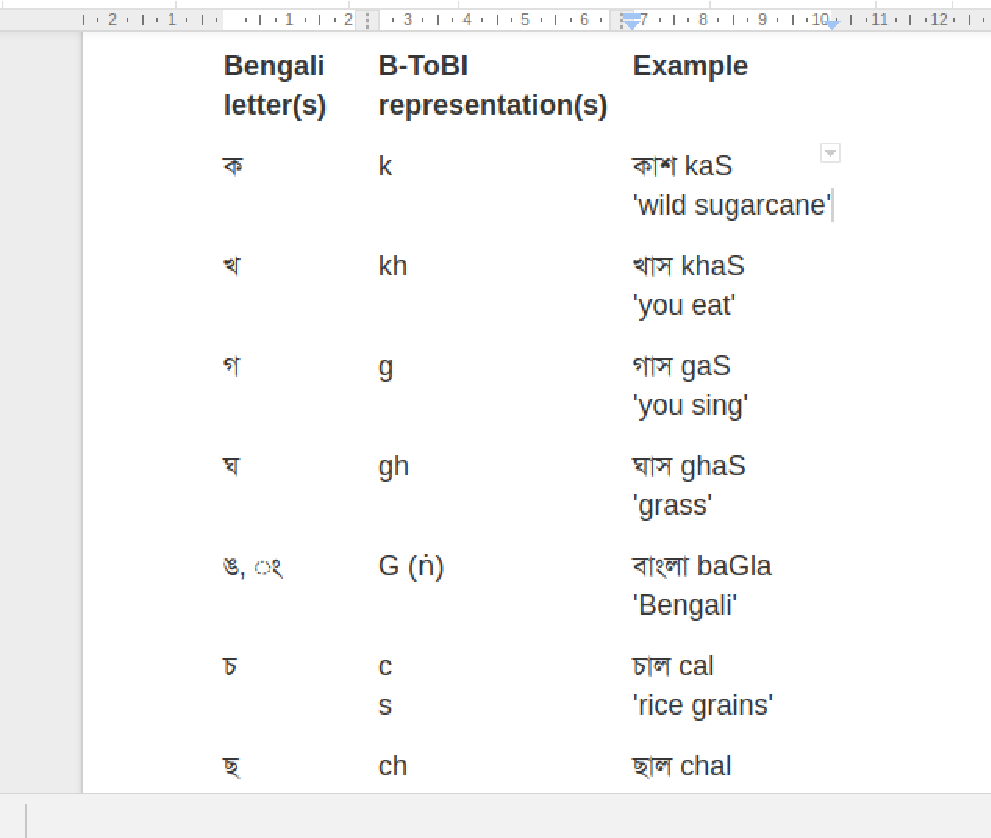
\includegraphics[width=13cm, height=5.5cm]{img/B-ToBI_phonemes.pdf}}
   \caption{B-ToBI Transcription}
  \label{fig:B-ToBI-transcription}
\end{figure}

\section{Building an ASR using DNN-HMM}
For DNN-HMM-based acoustic model in Bangla, we need a Bangla word corpus. We have collected 1035 isolated Bangla words from previous thesis works. Then we converted them to corresponding B-ToBI phonemes. Using this words and phonetic transcription we had to change some files to suit our model. These files are corpus.txt, lexicon.txt, nonsilence\_phones.txt, spk2gender.txt, spk2utt.txt, text.txt, utt2spk.txt, and wav.scp.
\\
After that, we train the DNN-HMM model in Kaldi that is mono-phone based. To train this model, it uses phoneme-to-audio alignments which were generated by a GMM-HMM system. So, it is needed to get a good alignment from the trained GMM-HMM model \cite{rabiner1989tutorial}.
\\
\subsection{DNN model selection}
We've used Kaldi's DNN implementation for training Deep Neural Network \cite{hinton2012deep}. There are two types of DNN implementation in Kaldi. The 1st one is a comparatively old training method
for DBN with pre-trained RBM (Restricted Boltzmann Machine). The other one is DNN
(greedy layer-wise supervised training). And the second one gave better performance in
several languages than the first one
\cite{zhang2014improving}.  We've used Kaldi's DNN that was greedy layer-wise supervised training with max out networks
(p-norm units, where p = 2). We've also used layer-wise backpropagation for training \cite{seide2011conversational}.

    \subsection{Building Model's Corpus}
  We have added all possible words and sentences from the unique isolated words in the dictionary. This corpus.txt file is located in the local folder of Kaldi. Here is an example of a sample corpus file.
    
    \begin{figure}[h]
 \centering
 \frame{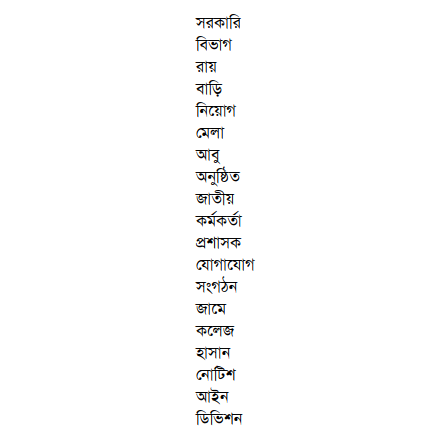
\includegraphics[width=13cm, height=7.5cm]{img/corpus}}
 \caption{corpus.txt sample file}
\label{fig:corpus}
\end{figure}

    
    \subsection{Dividing every words into Lexicon}
     This is a very important part of building a Kaldi model for any language. We've divided every word in its corresponding phonemes. Here we have used B-ToBI model of Bengali intonation. An example of our lexicon file is below:
\\  
         \begin{figure}[h]
 \centering
\frame{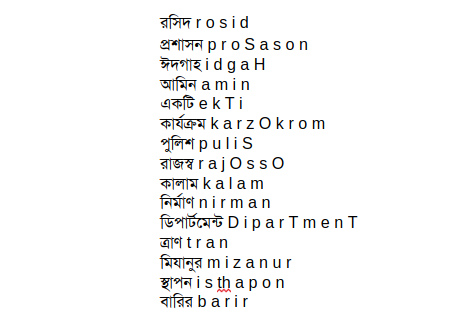
\includegraphics[width=13cm, height=6.5cm]{img/lexicon}}
 \caption{lexicon.txt sample file}
\label{fig:lexicon}
\end{figure}

       \subsection{Nonsilence unique phone}
    In this process, we have got 54 unique phones from B-ToBI technique. These phones are stored in nonsilence\_phones.txt file in Kaldi. These phones are used in lexicon.txt file and others. An example of a sample nonsilence phone list is below:
\\
   \begin{figure}[h]
 \centering
 \frame{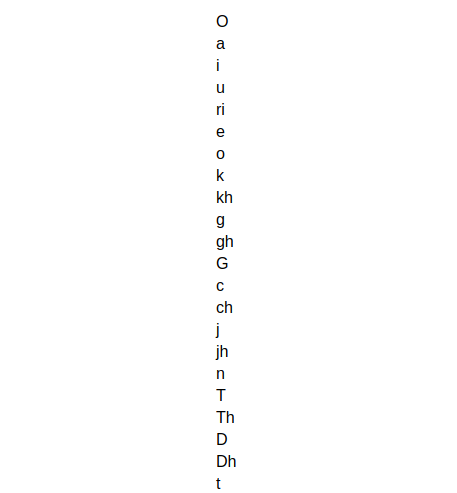
\includegraphics[width=15cm, height=6.5cm]{img/nonsilence_phones}}
 \caption{nonsilencephones.txt sample file}
\label{fig:nonsilence_phones}
\end{figure}

\subsection{Creating spk2gender.txt file}
Actually, we have worked on speaker dependent model in Kaldi that is DNN-HMM and other GMM-HMM models are speaker independent. So, we had to specify the gender of all acoustic signals that are the recorded voices. Here a sample of this file to know how to map the speaker to gender is below where 'f' means female and' means male: \\
It can be done just to make the speaker-ids the same as the utterance-ids if there are no information at all about the speaker identities.
So this file maps from speaker-id to either "m" or "f" depending on the speaker gender. All of these files must be sorted in Kaldi. If they are not sorted, there will be occurred errors when we run the run.sh script in Kaldi.

   \begin{figure}[h]
 \centering
 \frame{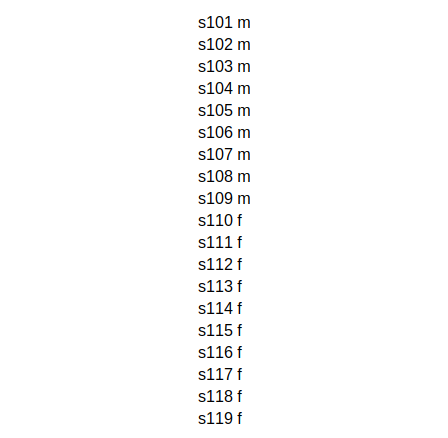
\includegraphics[width=15cm, height=6.0cm]{img/spk2gender}}
 \caption{spk2gender.txt sample file}
\label{fig:spk2gender}
\end{figure}

    \subsection{Building spk2utt and utt2spk}
  The spk2utt.txt file is the file for mapping the speaker and the utterance. And another one for the utterance to the speaker. These files are in Kaldi by default. Here are some of the examples we added:   \\   
   \begin{figure}[h]
 \centering
 \frame{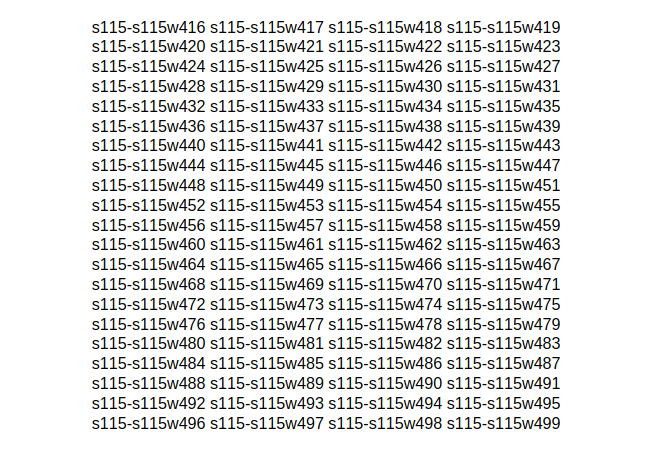
\includegraphics[width=15cm, height=6.9cm]{img/spk2utt}}
 \caption{spk2utt.txt sample file}
\label{fig:spk2utt}
\end{figure}    

    \begin{figure}[h]
 \centering
 \frame{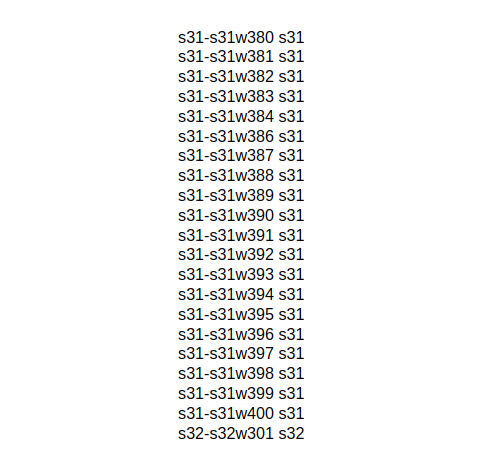
\includegraphics[width=13cm, height=7cm]{img/utt2spk}}
 \caption{utt2spk.txt sample file}
\label{fig:utt2spk}
\end{figure}
   
        
    \subsection{Creating text in train and test}
      There is the file called text.txt in each of the test and the train folder in the data section. This file maps among the speech file name and the 3 utterances. Here 3 utterance is for collecting the acoustic signal with 3 utterances of a word. Here are some of the examples:
    \\
   \begin{figure}[h]
 \centering
 \frame{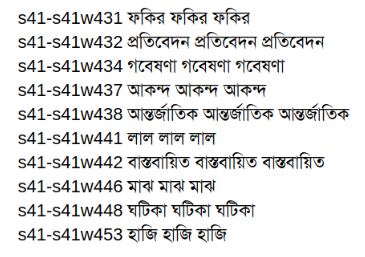
\includegraphics[width=13cm, height=5.5cm]{img/text}}
 \caption{text.txt sample file}
\label{fig:text.txt sample}
\end{figure}
            
    \subsection{Creating wav.scp file}
      There is another file included in the test and also in the train folder. Wav.scp file shows the file path of an acoustic voice or speech. Some examples are:
    \\
    \begin{figure}[h]
 \centering
 \frame{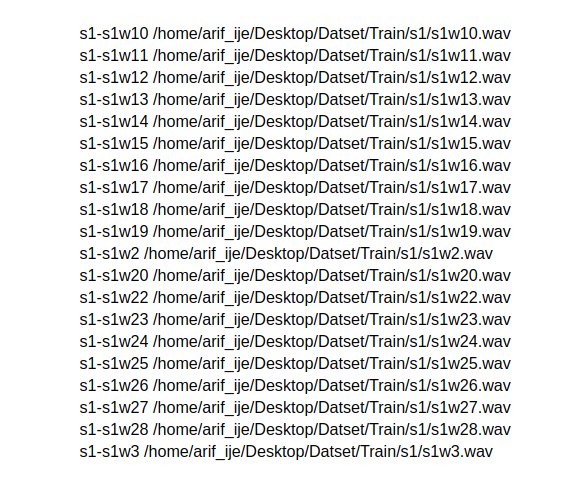
\includegraphics[width=13cm, height=7cm]{img/wavscp}}
 \caption{wav.scp sample file}
\label{fig:wavscp}
\end{figure}

\subsection{Feature Extraction}
To extract acoustic features from our collected acoustic signals or speeches we have used MFCC feature extraction technique.
It recognizes the parts of the sound flag with respect to silence phones that are useful for distinguishing the phonetic substances. No two words or utterances will not produce the same signal. Even the utterances of the same word are likely to produce the different digital signal. So, the target of the feature extraction phase is to derive a feature vector such that the vector for a similar phoneme is as near to each other.
Differences among speakers gender, dialect, pronunciation, voice, etc are the main elements that may cause two random speech samples to differ from each other. Feature extraction compresses the magnitude of the input signal(vector) without causing any harm to the power of speech signal.\\
Actually, MFCC extracts features such that the extracted signal is modified in the human cochlea. At first, it calculates the spectral density of the acoustic signals. Then it estimates Mel filterbank energy from each frame \cite{tiwari2010mfcc}. Then it also calculates the logarithm of the summation of all Mel filterbank energies for doing 8 times the loudness of the input signal. After all, it converts the all values in DCT form to decorrelates the energies. Here is an MFCC extraction process is shown below:
\\
\\
   \begin{figure}[h]
 \centering
 \frame{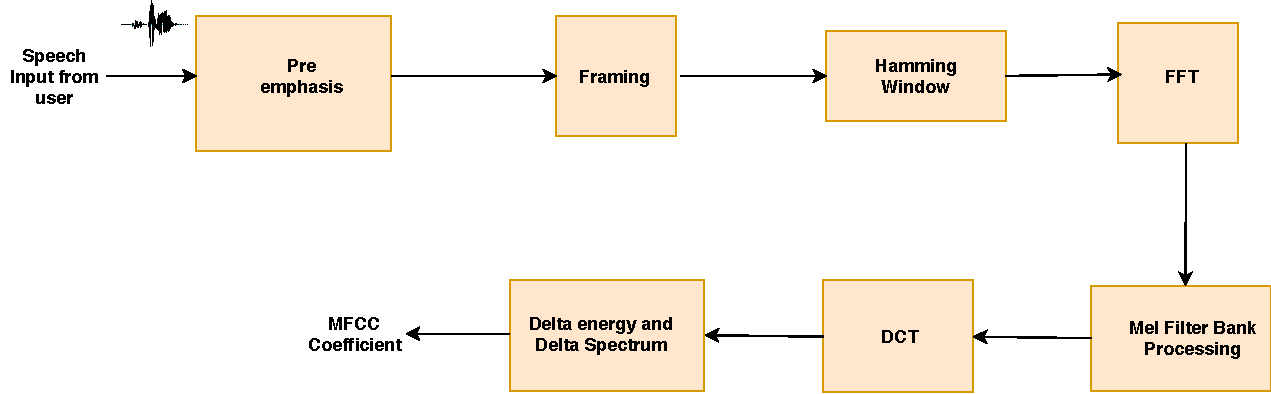
\includegraphics[width=13cm, height=6.5cm]{img/MFCC.pdf}}
 \caption{MFCC feature extraction process}
\label{fig:MFCC}
\end{figure}

 Now we've trained the model in Kaldi after completing the above all preprocessing steps. We can get an exp folder in the model directory where the models remain.

    
\end{document}